% !TeX program = xelatex
\documentclass[a4paper,10pt]{article}

% ============================================================================
% កញ្ចប់បណ្ណាល័យ (Packages) – តាមលំនាំ NGS Preah Krasang (ls_plan.tex)
% ============================================================================
\usepackage[a4paper, left=0.95cm, right=0.95cm, top=0.85cm, bottom=0.92cm, footskip=0.52cm]{geometry}
\usepackage{amsmath, amssymb}
\usepackage{unicode-math}
\usepackage{fontspec}
\usepackage{array, longtable, multirow, colortbl}
\usepackage[table]{xcolor}
\usepackage{enumitem}
\usepackage{pifont}
\usepackage{fancyhdr}
\usepackage{tikz}
\usetikzlibrary{calc, arrows.meta, angles, quotes, decorations.markings, patterns, babel}

% LaTeX 2025 + longtable v4.24 compatibility guard
\makeatletter
\let\@expl@@@mark@update@singlecol@structures@@\relax
\makeatother

% ============================================================================
% ការកំណត់ពុម្ពអក្សរ (Cross-Platform Windows + Cloud fonts/)
% ============================================================================
\providecommand{\NGSFindFonts}{%
  \IfFileExists{C:/Windows/Fonts/cambria.ttc}{%
    \def\NGSSysPath{C:/Windows/Fonts/}%
    \def\NGSUserPath{C:/Users/KIT/AppData/Local/Microsoft/Windows/Fonts/}%
  }{%
    \IfFileExists{./fonts/KhmerOSsiemreap.ttf}{\def\NGSSysPath{./fonts/}\def\NGSUserPath{./fonts/}}{%
    \IfFileExists{../fonts/KhmerOSsiemreap.ttf}{\def\NGSSysPath{../fonts/}\def\NGSUserPath{../fonts/}}{%
    \IfFileExists{../../fonts/KhmerOSsiemreap.ttf}{\def\NGSSysPath{../../fonts/}\def\NGSUserPath{../../fonts/}}{%
    \IfFileExists{../../../fonts/KhmerOSsiemreap.ttf}{\def\NGSSysPath{../../../fonts/}\def\NGSUserPath{../../../fonts/}}{%
    \IfFileExists{../../../../fonts/KhmerOSsiemreap.ttf}{\def\NGSSysPath{../../../../fonts/}\def\NGSUserPath{../../../../fonts/}}{%
    \IfFileExists{../../../../../fonts/KhmerOSsiemreap.ttf}{\def\NGSSysPath{../../../../../fonts/}\def\NGSUserPath{../../../../../fonts/}}{%
    \IfFileExists{../../../../../../fonts/KhmerOSsiemreap.ttf}{\def\NGSSysPath{../../../../../../fonts/}\def\NGSUserPath{../../../../../../fonts/}}{%
      \def\NGSSysPath{../../../../../../../fonts/}\def\NGSUserPath{../../../../../../../fonts/}%
    }}}}}}}%
  }%
}
\NGSFindFonts

\setmathfont[
  Path={\NGSSysPath},
  FontIndex=1,
  Scale=1.02
]{cambria.ttc}

\defaultfontfeatures{Ligatures=TeX}

\setmainfont[
  Path={\NGSUserPath},
  Extension=.ttf,
  Script=Khmer,
  BoldFont={KhmerOSsiemreap},
  BoldFeatures={FakeBold=1.8},
  ItalicFont={KhmerOSsiemreap},
  ItalicFeatures={FakeSlant=0.25},
  BoldItalicFont={KhmerOSsiemreap},
  BoldItalicFeatures={FakeBold=1.8, FakeSlant=0.25}
]{KhmerOSsiemreap}

\newfontfamily\muol[
  Path={\NGSUserPath},
  Extension=.ttf,
  Script=Khmer
]{KhmerOSmuollight}

\newfontfamily\TimesEn[
  Path={\NGSSysPath},
  Extension=.ttf,
  Scale=1.00,
  BoldFont={timesbd},
  ItalicFont={timesi},
  BoldItalicFont={timesbi}
]{times}

\newfontfamily\NagaBold[
  Path={\NGSUserPath},
  Extension=.ttf
]{AKbalthom Naga Bold}

\newfontfamily\CalibriFont[
  Path={\NGSSysPath},
  Extension=.ttf
]{calibri}

\newfontfamily\Tacteing[
  Path={\NGSUserPath}
]{TACTENG.TTF}

\newfontfamily\CourierBullet[
  Path={\NGSSysPath},
  Extension=.ttf
]{cour}
\newcommand{\wcirc}{{\CourierBullet\fontsize{9.5pt}{11pt}\selectfont o}}

\XeTeXlinebreaklocale "km"
\XeTeXlinebreakskip = 0pt plus 1pt minus 0.1pt

% ============================================================================
% ការកំណត់ពណ៌ និងទម្រង់ទំព័រ (Colors & Page Style)
% ============================================================================
\definecolor{stepgray}{HTML}{D9D9D9}
\definecolor{headgray}{HTML}{F2F2F2}
\definecolor{boxgray}{HTML}{D9D9D9}
\definecolor{darkred}{HTML}{C00000}
\definecolor{red5e}{HTML}{FF0000}

\pagestyle{fancy}
\fancyhf{}
\renewcommand{\headrulewidth}{0pt}
\fancyfoot[R]{\CalibriFont\fontsize{11pt}{13pt}\selectfont\thepage}

\setlength{\parindent}{0pt}
\setlength{\parskip}{0pt}
\setlength{\tabcolsep}{3.8pt}

\newcolumntype{L}[1]{>{\raggedright\arraybackslash}p{#1}}

% ============================================================================
% ម៉ាក្រូជំនួយ (Helper Macros)
% ============================================================================
\newcommand{\en}[1]{{\TimesEn #1}}
\newcommand{\enbf}[1]{{\TimesEn\textbf{#1}}}
\newcommand{\unit}[1]{\,\text{\en{#1}}}
\newcommand{\fiveE}[1]{{\NagaBold\fontsize{9.5pt}{13pt}\selectfont\textcolor{red5e}{#1}}}
\newcommand{\timenote}[1]{\textcolor{darkred}{\textit{#1}}}
\newcommand{\cnum}[1]{{\fontsize{10.5pt}{12pt}\selectfont\ding{\numexpr181+#1\relax}}\hspace{0.2em}}
\newcommand{\cfig}[1]{\par\vspace{4pt}{\centering #1\par}\vspace{4pt}}
\newcommand{\stepheader}[1]{\multicolumn{3}{|c|}{\cellcolor{stepgray}\muol #1} \\* \noalign{\hrule height 0.4pt}}
\newcommand{\tri}[1]{\ensuremath{\triangle #1}}
\newcommand{\ang}[1]{\ensuremath{\angle #1}}
\newcommand{\cg}{\ensuremath{\cong}}
\newcommand{\khmflourish}{{\Tacteing\fontsize{36pt}{14pt}\selectfont\raisebox{-5pt}{3}}}

\newcommand{\rightbox}[4][0.20cm]{%
  \draw[black, line width=0.8pt]
    ($(#3)!#1!(#2)$) -- ($($(#3)!#1!(#2)$)+($(#3)!#1!(#4)$)-(#3)$) -- ($(#3)!#1!(#4)$);
}

\tikzset{
  tk1/.style={postaction={decorate},decoration={markings,mark=at position 0.50 with {\draw[black, line width=0.85pt](0,-0.095)--(0,0.095);}}},
  tk2/.style={postaction={decorate},decoration={markings,
    mark=at position 0.45 with {\draw[black, line width=0.85pt](0,-0.095)--(0,0.095);},
    mark=at position 0.55 with {\draw[black, line width=0.85pt](0,-0.095)--(0,0.095);}}}
}

% ============================================================================
% ម៉ាក្រូរូបភាព TikZ ស-ខ្មៅ សមាមាត្រច្បាស់ (3.8 cm – 7.2 cm, អក្សរខ្មៅ 100%)
% ============================================================================

% ១. រូបបេសកកម្ម E1 (ស្រែចតុកោណកែង 8m x 3m ទល់នឹងស្រែប្រលេឡូក្រាម 8m, កម្ពស់ 3m, ជ្រុងទ្រេត 5m)
\newcommand{\figEngageAREAOne}{%
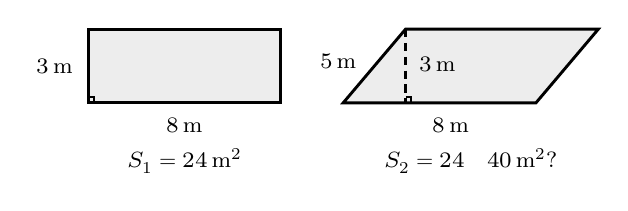
\begin{tikzpicture}[scale=0.36, every node/.style={font=\footnotesize, text=black}]
  % ស្រែទី ១ (ចតុកោណកែង)
  \begin{scope}[shift={(0,0)}]
    \fill[gray!14] (0,0) rectangle (6.8,2.6);
    \draw[black, line width=1.05pt] (0,0) rectangle (6.8,2.6);
    \rightbox[0.20cm]{0,2.6}{0,0}{6.8,0}
    \node[below=2pt] at (3.4,0) {$8\unit{m}$};
    \node[left=2pt] at (0,1.3) {$3\unit{m}$};
    \node at (3.5,1.3) {ស្រែទី១};
    \node[below=13pt] at (3.4,0) {$S_1 = 24\unit{m}^2$};
  \end{scope}
  % ស្រែទី ២ (ប្រលេឡូក្រាមទ្រេត)
  \begin{scope}[shift={(9.0,0)}]
    \coordinate (D) at (0,0);
    \coordinate (C) at (6.8,0);
    \coordinate (A) at (2.2,2.6);
    \coordinate (B) at (9.0,2.6);
    \coordinate (F) at (2.2,0);
    \fill[gray!14] (D) -- (C) -- (B) -- (A) -- cycle;
    \draw[black, line width=1.05pt] (D) -- (C) -- (B) -- (A) -- cycle;
    \draw[black, line width=0.85pt, densely dashed] (A) -- (F);
    \rightbox[0.20cm]{A}{F}{C}
    \node[below=2pt] at (3.8,0) {$8\unit{m}$};
    \node[left=1.5pt] at (0.95,1.45) {$5\unit{m}$};
    \node[right=1.5pt] at (2.2,1.35) {$3\unit{m}$};
    \node at (5.8,1.35) {ស្រែទី២};
    \node[below=13pt] at (4.5,0) {$S_2 = 24$ ឬ $40\unit{m}^2$?};
  \end{scope}
\end{tikzpicture}}

% ២. រូប E2 Contrasting Cases លើក្រឡាការេ៖ បំប្លែងប្រលេឡូក្រាម ABCD ទៅជាចតុកោណកែង ABEF
\newcommand{\figExploreGridAREAOne}{%
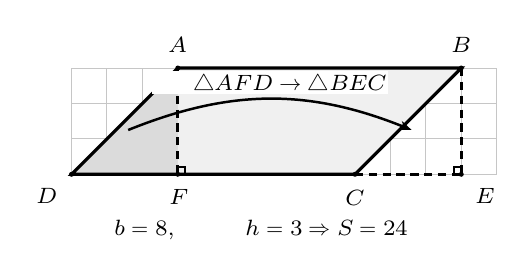
\begin{tikzpicture}[scale=0.45, every node/.style={font=\footnotesize, text=black}]
  \draw[gray!45, line width=0.35pt] (0,0) grid (12,3);
  \coordinate (D) at (0,0);
  \coordinate (F) at (3,0);
  \coordinate (C) at (8,0);
  \coordinate (E) at (11,0);
  \coordinate (A) at (3,3);
  \coordinate (B) at (11,3);
  \fill[gray!28] (D) -- (F) -- (A) -- cycle;
  \fill[gray!12] (F) -- (C) -- (B) -- (A) -- cycle;
  \draw[black, line width=1.15pt] (D) -- (C) -- (B) -- (A) -- cycle;
  \draw[black, line width=0.95pt, densely dashed] (A) -- (F) (B) -- (E) (C) -- (E);
  \rightbox[0.20cm]{A}{F}{C}
  \rightbox[0.20cm]{B}{E}{D}
  \draw[black, line width=0.9pt, -{Stealth[length=4.5pt]}, bend left=22] (1.6,1.25) to node[above=1.5pt, fill=white, inner sep=1pt] {រំកិល $\tri{AFD}\to\tri{BEC}$} (9.6,1.25);
  \fill[black] (A) circle (2.0pt) node[above=2pt] {$A$};
  \fill[black] (B) circle (2.0pt) node[above=2pt] {$B$};
  \fill[black] (D) circle (2.0pt) node[below left=1.5pt] {$D$};
  \fill[black] (F) circle (2.0pt) node[below=2pt] {$F$};
  \fill[black] (C) circle (2.0pt) node[below=2pt] {$C$};
  \fill[black] (E) circle (2.0pt) node[below right=1.5pt] {$E$};
  \node[below=13pt] at (5.8,0) {បាត $b=8$, កម្ពស់កែង $h=3 \Rightarrow S = 24$ ការេឯកតា};
\end{tikzpicture}}

% ៣. រូប E3 ទ្រឹស្តីបទប្រលេឡូក្រាម S = bh និងវិបាកត្រីកោណ S = 1/2 bh
\newcommand{\figExplainPairAREAOne}{%
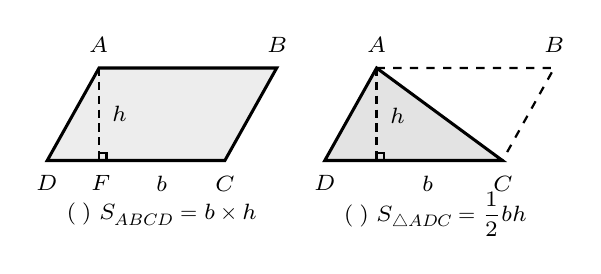
\begin{tikzpicture}[scale=0.47, every node/.style={font=\footnotesize, text=black}]
  \begin{scope}[shift={(0,0)}]
    \coordinate (D) at (0,0);
    \coordinate (C) at (4.8,0);
    \coordinate (A) at (1.4,2.5);
    \coordinate (B) at (6.2,2.5);
    \coordinate (F) at (1.4,0);
    \fill[gray!14] (D) -- (C) -- (B) -- (A) -- cycle;
    \draw[black, line width=1.1pt] (D) -- (C) -- (B) -- (A) -- cycle;
    \draw[black, line width=0.85pt, densely dashed] (A) -- (F);
    \rightbox[0.20cm]{A}{F}{C}
    \node[above=2pt] at (A) {$A$};
    \node[above=2pt] at (B) {$B$};
    \node[below=2pt] at (C) {$C$};
    \node[below=2pt] at (D) {$D$};
    \node[below=2pt] at (F) {$F$};
    \node[right=1.5pt] at (1.4,1.25) {$h$};
    \node[below=2pt] at (3.1,0) {$b$};
    \node at (3.1,-1.45) {(១) $S_{ABCD} = b \times h$};
  \end{scope}
  \begin{scope}[shift={(7.5,0)}]
    \coordinate (D) at (0,0);
    \coordinate (C) at (4.8,0);
    \coordinate (A) at (1.4,2.5);
    \coordinate (B) at (6.2,2.5);
    \coordinate (F) at (1.4,0);
    \fill[gray!22] (A) -- (D) -- (C) -- cycle;
    \draw[black, line width=1.1pt] (A) -- (D) -- (C) -- cycle;
    \draw[black, line width=0.8pt, dashed] (A) -- (B) -- (C);
    \draw[black, line width=0.85pt, densely dashed] (A) -- (F);
    \rightbox[0.20cm]{A}{F}{C}
    \node[above=2pt] at (A) {$A$};
    \node[above=2pt] at (B) {$B$};
    \node[below=2pt] at (C) {$C$};
    \node[below=2pt] at (D) {$D$};
    \node[right=1.5pt] at (1.4,1.2) {$h$};
    \node[below=2pt] at (2.8,0) {$b$};
    \node at (3.0,-1.45) {(២) $S_{\tri{ADC}} = \dfrac{1}{2}bh$};
  \end{scope}
\end{tikzpicture}}

% ៤. រូប E4 លំហាត់គំរូទី 1 & ទី 2 (ទំ. 189)
\newcommand{\figModelExAREAOne}{%
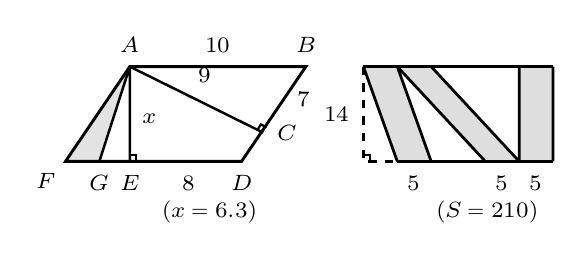
\begin{tikzpicture}[scale=0.43, every node/.style={font=\footnotesize, text=black}]
  \begin{scope}[shift={(0,0)}]
    \coordinate (F) at (0,0);
    \coordinate (G) at (1.0,0);
    \coordinate (E) at (1.9,0);
    \coordinate (D) at (5.2,0);
    \coordinate (A) at (1.9,2.8);
    \coordinate (B) at (7.1,2.8);
    \coordinate (C) at (5.84,0.85);
    \fill[gray!22] (A) -- (F) -- (G) -- cycle;
    \draw[black, line width=1.05pt] (F) -- (D) -- (B) -- (A) -- cycle;
    \draw[black, line width=0.9pt] (A) -- (G) (A) -- (E) (A) -- (C);
    \rightbox[0.19cm]{A}{E}{D}
    \rightbox[0.19cm]{A}{C}{B}
    \node[above=1.5pt] at (A) {$A$};
    \node[above=1.5pt] at (B) {$B$};
    \node[below left=1pt] at (F) {$F$};
    \node[below=1.5pt] at (G) {$G$};
    \node[below=1.5pt] at (E) {$E$};
    \node[below=1.5pt] at (D) {$D$};
    \node[right=1.5pt] at (C) {$C$};
    \node[above=1.5pt] at (4.5,2.8) {$10$};
    \node[right=1pt] at (1.9,1.25) {$x$};
    \node[above=1.5pt] at (4.1,1.9) {$9$};
    \node[right=1.5pt] at (6.45,1.85) {$7$};
    \node[below=1.5pt] at (3.65,0) {$8$};
    \node at (3.5,-1.50) {គំរូទី១ ($x=6.3$)};
  \end{scope}
  \begin{scope}[shift={(8.8,0)}]
    \coordinate (A) at (1.0,0);
    \coordinate (B) at (2.0,0);
    \coordinate (C) at (3.6,0);
    \coordinate (D) at (4.6,0);
    \coordinate (E) at (5.6,0);
    \coordinate (J) at (0,2.8);
    \coordinate (I) at (1.0,2.8);
    \coordinate (H) at (2.0,2.8);
    \coordinate (G) at (4.6,2.8);
    \coordinate (F) at (5.6,2.8);
    \fill[gray!26] (A) -- (B) -- (I) -- (J) -- cycle;
    \fill[gray!26] (C) -- (D) -- (H) -- (I) -- cycle;
    \fill[gray!26] (D) -- (E) -- (F) -- (G) -- cycle;
    \draw[black, line width=1.0pt] (J) -- (F) (A) -- (E);
    \draw[black, line width=1.0pt] (J)--(A) (I)--(B) (I)--(C) (H)--(D) (G)--(D) (F)--(E);
    \draw[black, line width=0.8pt, dashed] (J) -- (0,0) -- (A);
    \rightbox[0.19cm]{J}{0,0}{A}
    \node[left=1.5pt] at (0,1.4) {$14$};
    \node[below=1.5pt] at (1.5,0) {$5$};
    \node[below=1.5pt] at (4.1,0) {$5$};
    \node[below=1.5pt] at (5.1,0) {$5$};
    \node at (2.9,-1.50) {គំរូទី២ ($S=210$)};
  \end{scope}
\end{tikzpicture}}

% ៥. រូប E5 ប្រតិបត្តិ (ទំ. 190) + សំណួរវាយតម្លៃរហ័សត្រីកោណមុំទាល
\newcommand{\figPracticeEvalAREAOne}{%
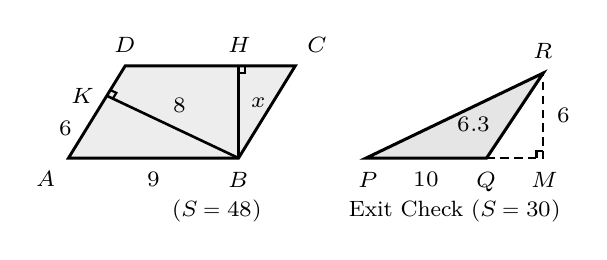
\begin{tikzpicture}[scale=0.45, every node/.style={font=\footnotesize, text=black}]
  \begin{scope}[shift={(0,0)}]
    \coordinate (A) at (0,0);
    \coordinate (B) at (4.8,0);
    \coordinate (D) at (1.6,2.6);
    \coordinate (C) at (6.4,2.6);
    \coordinate (H) at (4.8,2.6);
    \coordinate (K) at (1.08,1.76);
    \fill[gray!14] (A) -- (B) -- (C) -- (D) -- cycle;
    \draw[black, line width=1.05pt] (A) -- (B) -- (C) -- (D) -- cycle;
    \draw[black, line width=0.95pt] (B) -- (K) (B) -- (H);
    \rightbox[0.19cm]{B}{K}{D}
    \rightbox[0.19cm]{B}{H}{C}
    \node[below left=1pt] at (A) {$A$};
    \node[below=1.5pt] at (B) {$B$};
    \node[above right=1pt] at (C) {$C$};
    \node[above=1.5pt] at (D) {$D$};
    \node[above=1.5pt] at (H) {$H$};
    \node[left=1.5pt] at (K) {$K$};
    \node[below=1.5pt] at (2.4,0) {$9$};
    \node[left=1.5pt] at (0.5,0.85) {$6$};
    \node[above right=1pt] at (2.6,0.92) {$8$};
    \node[right=1.2pt] at (4.8,1.55) {$x$};
    \node at (3.2,-1.50) {ប្រតិបត្តិ ($S=48$)};
  \end{scope}
  \begin{scope}[shift={(8.4,0)}]
    \coordinate (P) at (0,0);
    \coordinate (Q) at (3.4,0);
    \coordinate (M) at (5.0,0);
    \coordinate (R) at (5.0,2.4);
    \fill[gray!20] (P) -- (Q) -- (R) -- cycle;
    \draw[black, line width=1.1pt] (P) -- (Q) -- (R) -- cycle;
    \draw[black, line width=0.85pt, densely dashed] (Q) -- (M) -- (R);
    \rightbox[0.19cm]{R}{M}{Q}
    \node[below=1.5pt] at (P) {$P$};
    \node[below=1.5pt] at (Q) {$Q$};
    \node[below=1.5pt] at (M) {$M$};
    \node[above=1.5pt] at (R) {$R$};
    \node[below=1.5pt] at (1.7,0) {$10$};
    \node[right=1.5pt] at (5.0,1.2) {$6$};
    \node[left=1.5pt] at (3.9,0.95) {$6.3$};
    \node at (2.5,-1.50) {\en{Exit Check} ($S=30$)};
  \end{scope}
\end{tikzpicture}}

% ============================================================================
% ចាប់ផ្ដើមឯកសារ (Document Body)
% ============================================================================
\begin{document}
\fontsize{10pt}{15.2pt}\selectfont

% -------------------- ក្បាលកិច្ចតែងការ (Header) --------------------
\begin{center}
  {\muol\fontsize{11pt}{16pt}\selectfont ព្រះរាជាណាចក្រកម្ពុជា}\\[2pt]
  {\muol\fontsize{10pt}{15pt}\selectfont ជាតិ សាសនា ព្រះមហាក្សត្រ}\\[1pt]
  \khmflourish
\end{center}

\vspace{-26pt}
{\muol\fontsize{9.5pt}{12.8pt}\selectfont
មន្ទីរអប់រំ យុវជន និងកីឡា ខេត្តកំពង់ធំ\\
ការិយាល័យអប់រំ យុវជន និងកីឡា ស្រុកកំពង់ស្វាយ\\
អនុវិទ្យាល័យព្រះក្រសាំង}

\vspace{1pt}
\begin{center}
  {\muol\fontsize{10pt}{14.5pt}\selectfont កិច្ចតែងការបង្រៀន}
\end{center}
\vspace{0pt}

% -------------------- ព័ត៌មានទូទៅ (Metadata) --------------------
{\renewcommand{\arraystretch}{0.98}
\hspace*{4.05cm}%
\begin{tabular}{@{}l l l@{}}
  - \hspace{0.35cm} មុខវិជ្ជា & : & គណិតវិទ្យា ថ្នាក់ទី៨ \\
  - \hspace{0.35cm} ចំណងជើងមេរៀន & : & មេរៀនទី១៤ ផ្ទៃក្រឡាពហុកោណ \\
  - \hspace{0.35cm} ចំណងជើងរង & : & ១. ផ្ទៃក្រឡាប្រលេឡូក្រាម (រួមទាំងវិបាកផ្ទៃក្រឡាត្រីកោណ ទំ.១៨៧--១៩០) \\
  - \hspace{0.35cm} រយៈពេល & : & ១ ម៉ោងសិក្សា (៥០ នាទី) \\
  - \hspace{0.35cm} បង្រៀនដោយ & : & ហុក ប៊ុនថែន \\
  - \hspace{0.35cm} កាលបរិច្ឆេទ & : & ថ្ងៃចន្ទ ទី១៤ ខែធ្នូ ឆ្នាំ២០២៦ \\
\end{tabular}

\vspace{2pt}

% -------------------- I. វត្ថុបំណង --------------------
\textbf{I.} {\muol វត្ថុបំណង}\\[1pt]
\hspace*{0.55cm}%
\begin{tabular}{@{}l l L{14.2cm}@{}}
  \wcirc \hspace{0.25cm} វិជ្ជាសម្បទា & : & សិស្សប្រាប់និយមន័យគូបាត--កម្ពស់កែង ($h \perp b$) ព្រមទាំងរូបមន្តផ្ទៃក្រឡាប្រលេឡូក្រាម ($S = bh$) និងត្រីកោណ ($S = \frac{1}{2}bh$) បានត្រឹមត្រូវតាមការប្រៀបធៀបករណីផ្ទុយគ្នាលើសន្លឹកកិច្ចការក្រឡាការេ ។ \\
  \wcirc \hspace{0.25cm} បំណិនសម្បទា & : & សិស្សស្រាយបញ្ជាក់ទ្រឹស្តីបទផ្ទៃក្រឡាប្រលេឡូក្រាម និងគណនាផ្ទៃក្រឡា ឬរង្វាស់កម្ពស់/បាតដែលបាត់តាមសមភាព $b_1h_1 = b_2h_2$ ទាំងទម្រង់ដេកនិងទម្រង់បង្វិលបាតបានត្រឹមត្រូវ ។ \\
  \wcirc \hspace{0.25cm} ចរិយាសម្បទា & : & សិស្សមានទម្លាប់ពិនិត្យសញ្ញាមុំកែង ($\perp$) មុនជ្រើសកម្ពស់ មិនច្រឡំជាមួយជ្រុងទ្រេត និងសហការផ្ទៀងផ្ទាត់សន្លឹកកិច្ចការជាដៃគូដោយហ្មត់ចត់ ។ \\
\end{tabular}

\vspace{2pt}

% -------------------- II. សម្ភារៈឧបទេស --------------------
\textbf{II.} {\muol សម្ភារៈឧបទេស}\\[1pt]
\hspace*{0.55cm}\parbox[t]{18.2cm}{$\bullet$ \hspace{0.25cm} សម្រាប់គ្រូ៖ សៀវភៅសិក្សាគោលគណិតវិទ្យាថ្នាក់ទី៨ (ទំ.១៨៧--១៩០ និង ១៩៤) ក្ដារខៀន ដីស បន្ទាត់វែង និងសន្លឹកកិច្ចការគំរូ (គ្មានស្លាយ \en{LCD}) ។\\
$\bullet$ \hspace{0.25cm} សម្រាប់សិស្ស៖ សន្លឹកកិច្ចការសិស្ស ស-ខ្មៅ (\en{Worksheet\_AREA1} ២ ទំព័រពេញ) សៀវភៅសិក្សាគោល សៀវភៅសរសេរ បន្ទាត់ក្រិត និងប៊ិច/ខ្មៅដៃ ។}

\vspace{2pt}

% -------------------- III. វិធីសាស្រ្តបង្រៀន --------------------
\textbf{III.} {\muol វិធីសាស្រ្តបង្រៀន}\\[1pt]
\hspace*{0.45cm}%
\begin{tabular}{@{}l l L{14.85cm}@{}}
  $\bullet$ \hspace{0.25cm} គោលវិធី & : & សិស្សមជ្ឈមណ្ឌល (បង្រៀនដោយមិនប្រើស្លាយ \en{LCD} យកសន្លឹកកិច្ចការបំពេញចន្លោះជាគោល) \\
  $\bullet$ \hspace{0.25cm} យុទ្ធវិធីបង្រៀន & : & ស្ថាបនានិយម គំរូ \en{5Es} រួមផ្សំការប្រៀបធៀបករណីផ្ទុយគ្នាលើក្រឡាការេ (\en{Contrasting Cases}) និងលំហាត់គំរូបំពេញចន្លោះតាមជំហាន (\en{Faded Worked Examples}) \\
\end{tabular}
}

\vspace{2pt}

% -------------------- IV. ដំណើរការបង្រៀន --------------------
\textbf{IV.} {\muol ដំណើរការបង្រៀន}

\vspace{1pt}

\renewcommand{\arraystretch}{1.15}
\begin{longtable}{|L{5.50cm}|L{7.90cm}|L{4.80cm}|}
\hline
\rowcolor{headgray}
\multicolumn{1}{|c|}{\muol សកម្មភាពគ្រូ} &
\multicolumn{1}{c|}{\muol ខ្លឹមសារមេរៀន} &
\multicolumn{1}{c|}{\muol សកម្មភាពសិស្ស} \\
\hline
\endfirsthead

\hline
\rowcolor{headgray}
\multicolumn{1}{|c|}{\muol សកម្មភាពគ្រូ} &
\multicolumn{1}{c|}{\muol ខ្លឹមសារមេរៀន} &
\multicolumn{1}{c|}{\muol សកម្មភាពសិស្ស} \\
\hline
\endhead

\hline
\endfoot

\hline
\endlastfoot

% ==================== ជំហានទី១ (2min) ====================
\stepheader{ជំហានទី១ ៖ រដ្ឋបាលថ្នាក់ (២ នាទី)}
$\bullet$ ពិនិត្យអវត្តមាន សណ្ដាប់ធ្នាប់ និងអនាម័យថ្នាក់រៀន\par\vspace{2pt}
$\bullet$ ចែកសន្លឹកកិច្ចការ \en{Worksheet\_AREA1} (១ សន្លឹកសងខាង) ដល់សិស្សគ្រប់គ្នា
&
$\bullet$ ពិនិត្យវត្តមាន និងការត្រៀមសម្ភារៈសិក្សា (សន្លឹកកិច្ចការ សៀវភៅសិក្សាគោល និងបន្ទាត់ក្រិត)
&
$\circ$ ប្រធានថ្នាក់រាយការណ៍អវត្តមាន\par\vspace{2pt}
$\circ$ ទទួលសន្លឹកកិច្ចការ និងសរសេរឈ្មោះ \\[3pt]
\hline

% ==================== ជំហានទី២ (9min: ≤3 + 3 + E1 3) ====================
\stepheader{ជំហានទី២ ៖ កែកិច្ចការផ្ទះ រំលឹកមេរៀនចាស់ និងភ្ជាប់មេរៀនថ្មី (៩ នាទី)}
\timenote{(កែកិច្ចការផ្ទះ $\le 3\unit{min}$)}\par\vspace{2pt}
$\bullet$ ហៅសិស្ស ១ នាក់ឡើងបំពេញចម្លើយសង្ខេបនៃលំហាត់ទី៥ (មេរៀនទី១៣ ទំ.១៨៥) លើក្ដារខៀន\par\vspace{2pt}
$\bullet$ ផ្ទៀងផ្ទាត់និងកែលម្អរហ័ស
&
\textbf{កំណែកិច្ចការផ្ទះ (មេរៀនទី១៣ ទំ.១៨៥)៖}\par\vspace{2pt}
ក្នុងប្រលេឡូក្រាម $ABCD$ បើ $\ang{A} = 65^\circ$ នោះ៖\par\vspace{2pt}
$\bullet$ មុំឈមប៉ុនគ្នា៖ $\ang{C} = \ang{A} = 65^\circ$\par\vspace{2pt}
$\bullet$ មុំតគ្នាបន្ថែមគ្នា៖ $\ang{B} = \ang{D} = 180^\circ - 65^\circ = 115^\circ$
&
$\circ$ សិស្ស ១ នាក់ឡើងសរសេរចម្លើយ\par\vspace{2pt}
$\circ$ សិស្សឯទៀតផ្ទៀងផ្ទាត់ក្នុងសៀវភៅសរសេរ \\[3pt]

\timenote{(រំលឹកមេរៀនទាក់ទង $3\unit{min}$)} $\bullet$ សំណួរទី១៖ «តើផ្ទៃក្រឡាចតុកោណកែង ($b, h$) គណនាតាមរូបមន្តអ្វី?»
&
\textbf{ចំណេះដឹងមូលដ្ឋានភ្ជាប់មេរៀនថ្មី៖} ១. ផ្ទៃក្រឡាចតុកោណកែង៖ $S = b \times h$ ($\unit{cm}^2, \unit{m}^2$) ។
&
$\circ$ ឆ្លើយ៖ «$S = b \times h$» \\[3pt]

\hspace*{0.3em}-- សំណួរទី២៖ «តើអង្កត់ទ្រូងមួយនៃប្រលេឡូក្រាមចែកវាជាត្រីកោណពីរយ៉ាងដូចម្ដេច?»
&
២. ទ្រឹស្ដីបទទី១ ប្រលេឡូក្រាម (ទំ.១៧១)៖ អង្កត់ទ្រូង $AC$ ចែកប្រលេឡូក្រាម $ABCD$ ជាត្រីកោណពីរប៉ុនគ្នា ($\tri{ABC} \cg \tri{CDA}$) ។
&
$\circ$ ឆ្លើយ៖ «ចែកជាត្រីកោណពីរប៉ុនគ្នា» \\[3pt]

\hspace*{0.3em}-- សំណួរទី៣៖ «រវាងអង្កត់កែង $AF$ និងអង្កត់ទ្រេត $AD$ គូសពី $A$ មកបន្ទាត់ $DC$ តើមួយណាខ្លីជាង?»
&
៣. អង្កត់កែងខ្លីជាងអង្កត់ទ្រេតជានិច្ច៖ $AF < AD$ កាលណា $AF \perp DC$ ។
&
$\circ$ ឆ្លើយ៖ «អង្កត់កែង $AF$ ខ្លីជាងអង្កត់ទ្រេត $AD$» \\[3pt]

\fiveE{E1 - Engage} \timenote{(3 min)}\par\vspace{1pt}
$\bullet$ ឱ្យសិស្សពិនិត្យ \textbf{ផ្នែកទី១} លើសន្លឹកកិច្ចការ (បេសកកម្មវាស់ដីស្រែពីរក្បែរប្រឡាយទឹកព្រះក្រសាំង)
&
\textbf{បេសកកម្ម E1៖ ដីស្រែពីរក្បែរប្រឡាយទឹក}\par\vspace{1pt}
$\bullet$ ស្រែទី១ (ចតុកោណកែង)៖ $S_1 = 8 \times 3 = 24\unit{m}^2$ ។\par\vspace{1pt}
$\bullet$ ស្រែទី២ (ប្រលេឡូក្រាម)៖ បាត $8\unit{m}$, គម្លាតកែង $3\unit{m}$, ភ្លឺទ្រេត $5\unit{m}$ ។
&
$\circ$ អានស្ថានភាពលើសន្លឹកកិច្ចការ \\[3pt]

\hspace*{0.3em}-- សំណួរ៖ «ពូសុខថា ស្រែទី២ ធំជាង ព្រោះ $8\times 5 = 40\unit{m}^2$ ។ តើប្អូនយល់ស្រប ឬទេ?»
&
$\bullet$ សំណួរគន្លឹះ៖ តើ $S_2 = 40\unit{m}^2$ ឬ $S_2 = 24\unit{m}^2$? (ទុកផ្ទៀងនៅ E5)
&
$\circ$ គូសធីក $\square$ ទស្សន៍ទាយមុនរៀនដោយសេរីលើសន្លឹកកិច្ចការ \\[3pt]

& \cfig{\figEngageAREAOne} & \\[3pt]
\hline

% ==================== ជំហានទី៣ (17min: E2 11 + E3 6) ====================
\stepheader{ជំហានទី៣ ៖ មេរៀនថ្មី — ១. ផ្ទៃក្រឡាប្រលេឡូក្រាម និងត្រីកោណ (១៧ នាទី)}
\fiveE{E2 - Explore} \timenote{(11 min)}\par\vspace{1pt}
$\bullet$ ណែនាំសិស្សធ្វើការជាដៃគូ (តុជាប់គ្នា) លើ \textbf{ផ្នែកទី២ នៃសន្លឹកកិច្ចការ} (\en{Contrasting Cases})
&
\textbf{សកម្មភាពរុករកលើសន្លឹកកិច្ចការក្រឡាការេ (ទំ.១៨៧--១៨៨)៖}\par\vspace{1pt}
$\bullet$ \textbf{ករណី A (ចតុកោណកែងគោល)៖} បណ្ដោយ $8$ ឯកតា, ទទឹងកែង $3$ ឯកតា $\Rightarrow$ រាប់ក្រឡាបាន $24$ ការេឯកតា ។
&
$\circ$ ពិភាក្សាជាដៃគូលើសន្លឹកកិច្ចការ \\[3pt]

$\bullet$ ឱ្យសិស្សគូសឆ្នូតលើ $\tri{AFD}$ ខាងឆ្វេង រួចគូសព្រួញរំកិលទៅបំពេញ $\tri{BEC}$ ខាងស្ដាំ និងរាប់ក្រឡាការេសរុប
&
$\bullet$ \textbf{ករណី B (ប្រលេឡូក្រាម $ABCD$)៖} បាត $DC = 8$, កម្ពស់កែង $AF = BE = 3$, ជ្រុងទ្រេត $AD = BC = 5$ ។\par\vspace{1pt}
$\bullet$ ពេលកាត់ $\tri{AFD}$ រំកិលទៅដាក់លើ $\tri{BEC}$ គេបានចតុកោណកែងថ្មី $ABEF$ មានបាត $8$ និងទទឹងកែង $3$ ។
&
$\circ$ គូសឆ្នូតលើ $\tri{AFD}$ និងផ្ទៀងធាតុត្រូវគ្នានៃ $\tri{AFD}$ និង $\tri{BEC}$\par\vspace{1pt}
$\circ$ រាប់ក្រឡារបស់ $ABEF$ ឃើញស្មើ $24$ ក្រឡាដូចករណី A \\[3pt]

& \cfig{\figExploreGridAREAOne} & \\[3pt]

$\bullet$ ដើរពិនិត្យតាមតុ និងសួរសំណួរអន្ទាក់ទី១៖ «ហេតុអ្វីផលគុណ $8 \times 5 = 40$ មិនមែនជាផ្ទៃក្រឡារបស់ប្រលេឡូក្រាម $ABCD$?»
&
\textbf{ការបំបែកអន្ទាក់ការយល់ច្រឡំ៖} ជ្រុង $AD = 5$ ជា \textbf{ជ្រុងទ្រេត} (មិនកែងនឹងបាត $DC$) ។ បើបត់ប្រលេឡូក្រាមឱ្យកាន់តែទ្រេត ជ្រុង $5$ នៅដដែល តែកម្ពស់កែង $h$ កាន់តែទាប ហើយផ្ទៃក្រឡាកាន់តែតូច! ត្រូវគុណបាតនឹង \textbf{កម្ពស់កែង $h$} ជានិច្ច ។
&
$\circ$ បកស្រាយហេតុផល៖ «ព្រោះ $5$ ជាជ្រុងទ្រេត មិនកែងនឹងបាត $8$ ទេ!» \\[3pt]

$\bullet$ សំណួរទី២៖ «បើគូសអង្កត់ទ្រូង $AC$ ពុះប្រលេឡូក្រាម $ABCD$ ជាពីរ តើផ្ទៃក្រឡា $\tri{ADC}$ ស្មើប៉ុន្មានភាគនៃផ្ទៃប្រលេឡូក្រាម?»
&
$\bullet$ \textbf{ករណី C (ពុះតាមអង្កត់ទ្រូង $AC$)៖} ដោយ $\tri{ADC} \cg \tri{CBA}$ (ជ.ជ.ជ) នោះផ្ទៃក្រឡាត្រីកោណនីមួយៗស្មើពាក់កណ្ដាលផ្ទៃប្រលេឡូក្រាម៖ $S_{\tri{ADC}} = \frac{1}{2} \times 24 = 12$ ការេឯកតា ។
&
$\circ$ ឆ្លើយ៖ «ផ្ទៃត្រីកោណស្មើពាក់កណ្ដាលផ្ទៃប្រលេឡូក្រាម គឺ $\frac{1}{2}bh$» \\[3pt]

\fiveE{E3 - Explain} \timenote{(6 min)}\par\vspace{1pt}
$\bullet$ ហៅតំណាងដៃគូបង្ហាញលទ្ធផល រួចគ្រូសរសេរទ្រឹស្ដីបទ និងសម្រាយបញ្ជាក់លើក្ដារខៀន (កែសម្រួលនិមិត្តសញ្ញាទំ.១៨៨ ពី $\cg$ មក $=$ សម្រាប់ផ្ទៃក្រឡា)
&
\textbf{១. ផ្ទៃក្រឡាប្រលេឡូក្រាម (ទំ.១៨៨)៖}\par\vspace{1pt}
$\bullet$ \textbf{ទ្រឹស្ដីបទ៖} ផ្ទៃក្រឡាប្រលេឡូក្រាមដែលមានបាត $b$ និងកម្ពស់ $h$ កំណត់ដោយរូបមន្ត៖ $S = bh$ ។
&
$\circ$ បំពេញប្រអប់ទ្រឹស្ដីបទលើសន្លឹកកិច្ចការ \\[3pt]

$\bullet$ ណែនាំឱ្យសិស្សបំពេញសម្រាយបញ្ជាក់សង្ខេបក្នុង \textbf{ផ្នែកទី៣} នៃសន្លឹកកិច្ចការ
&
$\bullet$ \textbf{សម្រាយបញ្ជាក់៖} គូស $AF \perp DC$ និង $BE \perp DC$ (បន្លាយ) ។ ក្នុងត្រីកោណកែង $\tri{AFD}$ និង $\tri{BEC}$ មាន $AD = BC$ និង $AF = BE = h$ នាំឱ្យ $\tri{AFD} \cg \tri{BEC}$ (អ.ជ) $\Rightarrow S_{\tri{AFD}} = S_{\tri{BEC}}$ ។ គេបាន $S_{ABCD} = S_{ABCF} + S_{\tri{AFD}} = S_{ABCF} + S_{\tri{BEC}} = S_{ABEF} = b \times h$ ។
&
$\circ$ បំពេញជំហានសម្រាយបញ្ជាក់ និងកត់សម្គាល់ថា $\cg$ សម្រាប់រូបប៉ុនគ្នា រីឯ $=$ សម្រាប់ទំហំផ្ទៃស្មើគ្នា \\[3pt]

& \cfig{\figExplainPairAREAOne} & \\[3pt]

$\bullet$ បញ្ជាក់បន្ថែមលើវិបាកត្រីកោណ ឧទាហរណ៍ទំ.១៨៨ និងធនាគារហេតុផល \cnum{1}--\cnum{4}
&
$\bullet$ \textbf{សម្គាល់ (ផ្ទៃក្រឡាត្រីកោណ)៖} $S = \dfrac{1}{2} b \times h$ ។ \textbf{ឧទាហរណ៍៖} បើ $b = 8\unit{cm}, h = 3\unit{cm}$ នោះ $S_{\text{ប្រលេឡូក្រាម}} = 24\unit{cm}^2$ និង $S_{\tri{}} = 12\unit{cm}^2$ ។\par\vspace{1pt}
$\bullet$ \textbf{ធនាគារហេតុផល៖} \cnum{1} $h \perp b$ \;\vert\; \cnum{2} $S = bh$ \;\vert\; \cnum{3} $b_1h_1 = b_2h_2$ \;\vert\; \cnum{4} $S_{\tri{}} = \frac{1}{2}bh$ ។
&
$\circ$ គណនាឧទាហរណ៍ផ្ទាល់មាត់ និងគូសរង្វង់សម្គាល់សមភាព \cnum{3} ($b_1h_1 = b_2h_2$) លើសន្លឹកកិច្ចការ \\[3pt]
\hline

% ==================== ជំហានទី៤ (20min: E4 10 + E5 10) ====================
\stepheader{ជំហានទី៤ ៖ ពង្រីកចំណេះដឹង និងវាយតម្លៃ (២០ នាទី)}
\fiveE{E4 - Elaborate} \timenote{(10 min)}\par\vspace{1pt}
$\bullet$ ដឹកនាំសិស្សបំពេញ \textbf{ផ្នែកទី៤ (\en{Faded Worked Examples})} តាមសៀវភៅគោលទំ.១៨៩
&
\textbf{លំហាត់គំរូទី ១ (ទំ.១៨៩)៖} គេមានប្រលេឡូក្រាម $ABDF$ មាន $AB = FD = 10\unit{cm}$, $BD = 7\unit{cm}$, $AC = 9\unit{cm}$ ($AC \perp BD$), $AE = x$ ($AE \perp FD$) និង $ED = 8\unit{cm}$ ។
&
$\circ$ គូសរង្វង់សម្គាល់មុំកែងត្រង់ $E$ ($FD \perp AE$) និងត្រង់ $C$ ($BD \perp AC$) \\[3pt]

$\bullet$ ណែនាំ \textbf{[tracing]}៖ ផ្គូផ្គងគូបាត--កម្ពស់មុនជំនួសលេខក្នុងសំណួរ ក.
&
\textbf{ក. គណនាតម្លៃ $x$ ៖} តាមហេតុផល \cnum{3} ($FD \times AE = BD \times AC$)\par\vspace{1pt}
$10 \times x = 7 \times 9 \implies x = \dfrac{63}{10} = 6.3\unit{cm}$ ។
&
$\circ$ បំពេញជំហានគណនា $x = 6.3\unit{cm}$ លើសន្លឹកកិច្ចការ \\[3pt]

$\bullet$ ដឹកនាំសំណួរ ខ. (បញ្ជាក់កែកំហុសបោះពុម្ពទំ.១៨៩ ដែលសរសេរ $AGF$ ជំនួស $AGE$)
&
\textbf{ខ. គណនា $S_{\tri{AFG}}$ បើដឹងថា $S_{\tri{AGE}} = 3.15\unit{cm}^2$ ៖} $FE = FD - ED = 10 - 8 = 2\unit{cm}$ ។\par\vspace{1pt}
តាម \cnum{4}៖ $S_{\tri{AFE}} = \dfrac{1}{2} \times 2 \times 6.3 = 6.3\unit{cm}^2 \implies S_{\tri{AFG}} = 6.3 - 3.15 = 3.15\unit{cm}^2$ ។
&
$\circ$ បំពេញចម្លើយ $S_{\tri{AFG}} = 3.15\unit{cm}^2$ លើសន្លឹកកិច្ចការ \\[3pt]

& \cfig{\figModelExAREAOne} & \\[3pt]

$\bullet$ ឱ្យសិស្សបំពេញបន្ត \textbf{លំហាត់គំរូទី ២ (ទំ.១៨៩)} ដោយខ្លួនឯង (Faded Step ចុងក្រោយ)
&
\textbf{លំហាត់គំរូទី ២ (ទំ.១៨៩)៖} បន្ទះប្រលេឡូក្រាមប្រផេះទាំង ៣ មានបាតស្មើគ្នា $b = 5\unit{cm}$ និងកម្ពស់កែងរួម $h = 14\unit{cm}$ ៖ $S = 3 \times (5 \times 14) = 3 \times 70 = 210\unit{cm}^2$ ។
&
$\circ$ បំពេញប្រអប់ចម្លើយ $S = 210\unit{cm}^2$ \\[3pt]

$\bullet$ សួរសំណួរឆ្លុះបញ្ចាំង (\en{Looking-Back})៖ «ហេតុអ្វីបន្ទះកណ្ដាលទ្រេតខ្លាំង តែនៅតែមានផ្ទៃស្មើបន្ទះពីរទៀត?»
&
$\bullet$ \textbf{ចំណុចឆ្លុះបញ្ចាំង៖} ប្រលេឡូក្រាមមានបាតស្មើគ្នា និងកម្ពស់កែងស្មើគ្នា តែងមានផ្ទៃក្រឡាស្មើគ្នាជានិច្ច ។
&
$\circ$ ឆ្លើយ៖ «ព្រោះវាមានបាត $5\unit{cm}$ និងកម្ពស់កែងរួម $14\unit{cm}$ ដូចគ្នា!» \\[3pt]

\fiveE{E5 - Evaluate} \timenote{(10 min)}\par\vspace{1pt}
$\bullet$ ឱ្យសិស្សធ្វើ \textbf{ប្រតិបត្តិ (ទំ.១៩០)} ក្នុង \textbf{ផ្នែកទី៥} តាមទម្រង់ \textbf{ធ្វើទោល ៤ នាទី $\to$ ផ្ទៀងផ្ទាត់ដៃគូ ៣ នាទី (\en{Think-Pair-Check})}
&
\textbf{ប្រតិបត្តិ (ទំ.១៩០)៖} $ABCD$ ជាប្រលេឡូក្រាមមាន $AB = DC = 9\unit{cm}$, $AD = 6\unit{cm}$, $BK = 8\unit{cm}$ ($BK \perp AD$) និង $BH = x$ ($BH \perp DC$) ៖\par\vspace{1pt}
$\bullet$ \textbf{ក. ផ្ទៃក្រឡា $ABCD$ ៖} $S_{ABCD} = AD \times BK = 6 \times 8 = 48\unit{cm}^2$ (មិនមែន $9 \times 8$ ទេ!) ។
&
$\circ$ គណនាដោយខ្លួនឯងលើសន្លឹកកិច្ចការ រួចប្ដូរពិនិត្យជាមួយដៃគូ \\[3pt]

$\bullet$ ហៅសិស្ស ២ នាក់ឡើងបង្ហាញចម្លើយ ក. និង ខ. លើក្ដារខៀន
&
$\bullet$ \textbf{ខ. តម្លៃ $x$ ៖} តាម $DC \times BH = S_{ABCD} \implies 9 \times x = 48 \implies x = \dfrac{48}{9} = \dfrac{16}{3}\unit{cm} \approx 5.33\unit{cm}$ ។
&
$\circ$ ផ្ទៀងផ្ទាត់ការចាប់គូ $AD \perp BK$ និង $DC \perp BH$ \\[3pt]

& \cfig{\figPracticeEvalAREAOne} & \\[3pt]

$\bullet$ បិទបញ្ចប់បេសកកម្ម E1 និងធ្វើតេស្តរហ័ស ៩០ វិនាទី (\textbf{Exit Check ៤ ជម្រើស A/B/C/D})៖ លើកម្រាមដៃ ១--៤ តំណាងចម្លើយ A--D
&
\textbf{បិទបេសកកម្ម E1៖} ស្រែទាំងពីរមានផ្ទៃក្រឡាស្មើគ្នា $S_1 = S_2 = 8 \times 3 = 24\unit{m}^2$ ។\par\vspace{1pt}
\textbf{Exit Check ($\tri{PQR}$ បាត $PQ=10\unit{cm}$, កម្ពស់ក្រៅ $RM=6\unit{cm}$, ជ្រុងទ្រេត $6.3\unit{cm}$)៖} A. $60\unit{cm}^2$ \;\vert\; \textbf{B. $30\unit{cm}^2$ (ត្រូវ)} \;\vert\; C. $31.5\unit{cm}^2$ \;\vert\; D. $63\unit{cm}^2$ ។
&
$\circ$ លើកម្រាមដៃទី២ ជ្រើសចម្លើយ \textbf{B ($30\unit{cm}^2$)} និងពន្យល់ថា $RM \perp PQ$ (បន្លាយ) ជាកម្ពស់កែង \\[3pt]
\hline

% ==================== ជំហានទី៥ (≤2min) ====================
\stepheader{ជំហានទី៥ ៖ កិច្ចការផ្ទះ និងបណ្ដាំផ្ញើ ($\le$ ២ នាទី)}
\timenote{(ចំណាយពេល $\le 2\unit{min}$)}\par\vspace{2pt}
$\bullet$ ដាក់កិច្ចការផ្ទះពីសៀវភៅគោលទំ.១៩៤ (មានបោះពុម្ពជូនស្រាប់នៅបាតសន្លឹកកិច្ចការ)\par\vspace{2pt}
$\bullet$ ផ្ដាំផ្ញើឱ្យអានមុនចំណុច \textbf{២. ផ្ទៃក្រឡាចតុកោណស្មើ (ទំ.១៩០--១៩១)}
&
\textbf{កិច្ចការផ្ទះ (សៀវភៅសិក្សាគោល ទំព័រ ១៩៤)៖}\par\vspace{2pt}
១. \textbf{លំហាត់ទី ១ (ក, ខ, គ)៖} បំពេញតារាងបាត កម្ពស់ និងផ្ទៃក្រឡាប្រលេឡូក្រាម ៖ (ក) $b=12, h=7 \Rightarrow S=?$ ; (ខ) $h=6, S=42 \Rightarrow b=?$ ; (គ) $b=7.8, S=42.9 \Rightarrow h=?$ ។\par\vspace{2pt}
២. \textbf{លំហាត់ទី ២ (រូបទី១)៖} ប្រលេឡូក្រាម $SRQP$ មានបាត $PQ=SR=28\unit{cm}$, កម្ពស់ $SH=7\unit{cm}$, ជ្រុង $RQ=SP=8\unit{cm}$ និងកម្ពស់ $PR=x$ ($PR\perp RQ$) គណនាតម្លៃ $x$ ។
&
$\circ$ កត់ត្រានិងពិនិត្យប្រអប់កិច្ចការផ្ទះលើសន្លឹកកិច្ចការ\par\vspace{2pt}
$\circ$ ទទួលបណ្ដាំផ្ញើ និងជម្រាបលាគ្រូ \\[3pt]
\end{longtable}

% -------------------- កាលបរិច្ឆេទ និងហត្ថលេខា --------------------
\vspace{14pt}
\hfill
\begin{minipage}{9.8cm}
  {\centering
    ថ្ងៃចន្ទ ៥កើត ខែមិគសិរ ឆ្នាំមមី អដ្ឋស័ក ពុទ្ធសករាជ ២៥៧០\\[2pt]
    ព្រះក្រសាំង, ថ្ងៃទី១៤ ខែធ្នូ ឆ្នាំ២០២៦\\[3pt]
    {\muol គ្រូបង្រៀន}\par}
  \vspace{32pt}
  \hfill{\muol ហុក ប៊ុនថែន}\hspace*{1.4cm}
\end{minipage}

\end{document}
